\section{Ejemplos} 
Encuentre  las raíces de los siguientes polinomios utilizando Newton-Rahpson y muestre el gradiente de convergencia de la función:


\textbf{Función:}$x^7-x-1$

\textbf{Raíces:}

\begin{center}
\begin{tabular}{ c c }
 (-0.8099-0.2629i) & (-0.8099+0.2629i) \\
 (-0.3636-0.9526i) & (-0.3636+0.9526i) \\
 (0.6171-0.9009i) & (0.6171-0.9009i) \\  
 (1.1128-0i)  
\end{tabular}
\end{center}


\begin{figure}[H]
    \centering
    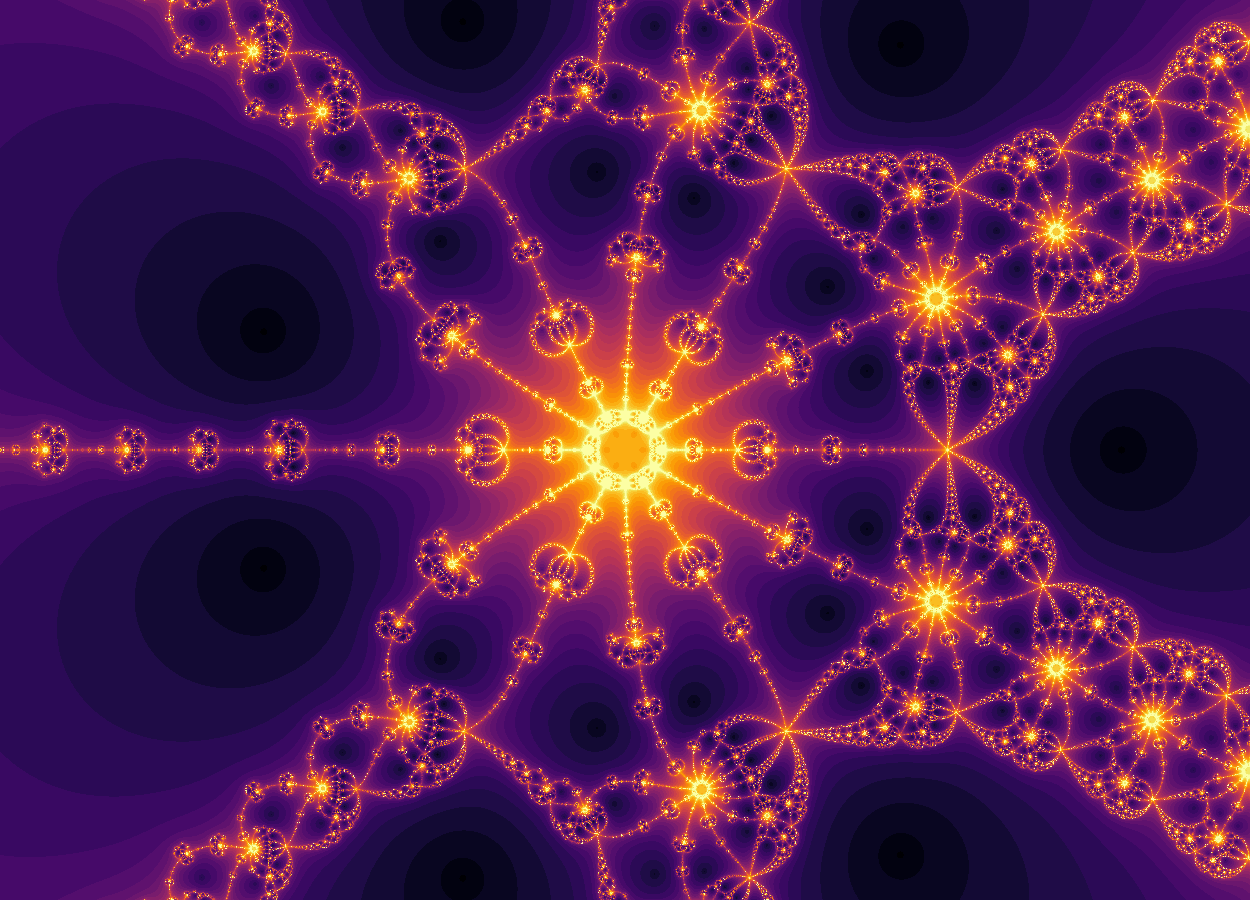
\includegraphics[scale=0.26]{images/ej1.png}
    \caption{Fractal generado por $x^7-x-1$}
    \label{fig:ej_1}
\end{figure}

\textbf{Función:}$x^6-x^3+11$

\textbf{Raíces:}

\begin{center}
\begin{tabular}{ c c }
 (-1.2523-0.8098i) & (-1.2523+0.8098i) \\
 (-0.0752-1.4894i) & (-0.0752+1.4894i) \\
 (1.3275-0.6796i) & (1.3275+0.6796i)
\end{tabular}
\end{center}

\begin{figure}[H]
    \centering
    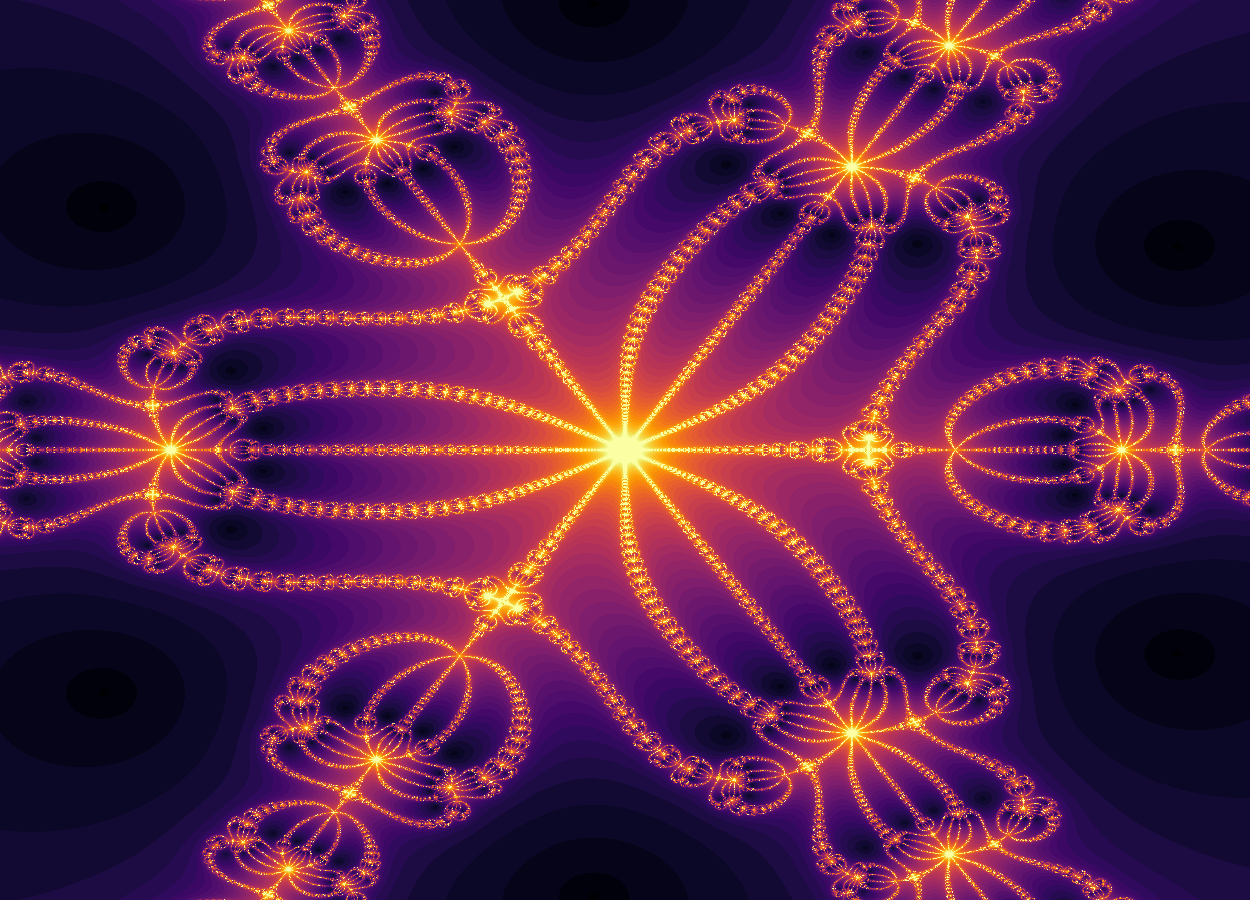
\includegraphics[scale=0.26]{images/ej2.png}
    \caption{Fractal generado por $x^6-x^3+11$}
    \label{fig:ej_2}
\end{figure}

\textbf{Función:}$x^4-x^2-1$

\textbf{Raíces:}

\begin{center}
\begin{tabular}{ c c  }
 (-1.272+0i) & (-0-0.7862i) \\
 0.7862i & (1.272+0i)
\end{tabular}
\end{center}

\begin{figure}[H]
    \centering
    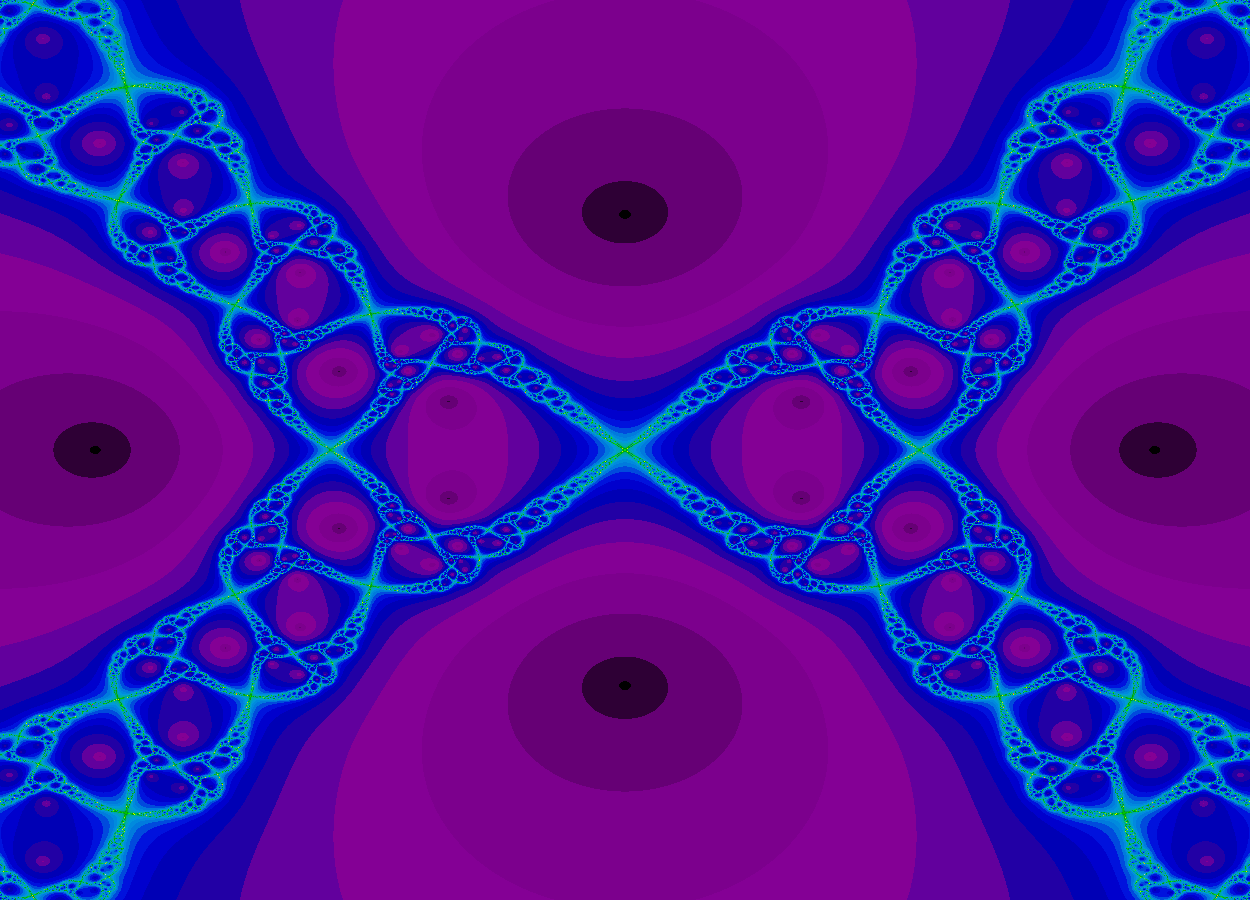
\includegraphics[scale=0.26]{images/ej3.png}
    \caption{Fractal generado por $x^4-x^2-1$}
    \label{fig:ej_3}
\end{figure}

\textbf{Función:}$x^6-3x^2-2x$

\textbf{Raíces:}

\begin{center}
\begin{tabular}{ c c  }
    (-1+0i) & (-0.7413+0i) \\ 
    0i & (0.1472-1.3576i) \\ 
    (0.1472+1.3576i) & (1.4469+0i)
 
\end{tabular}
\end{center}

\begin{figure}[H]
    \centering
    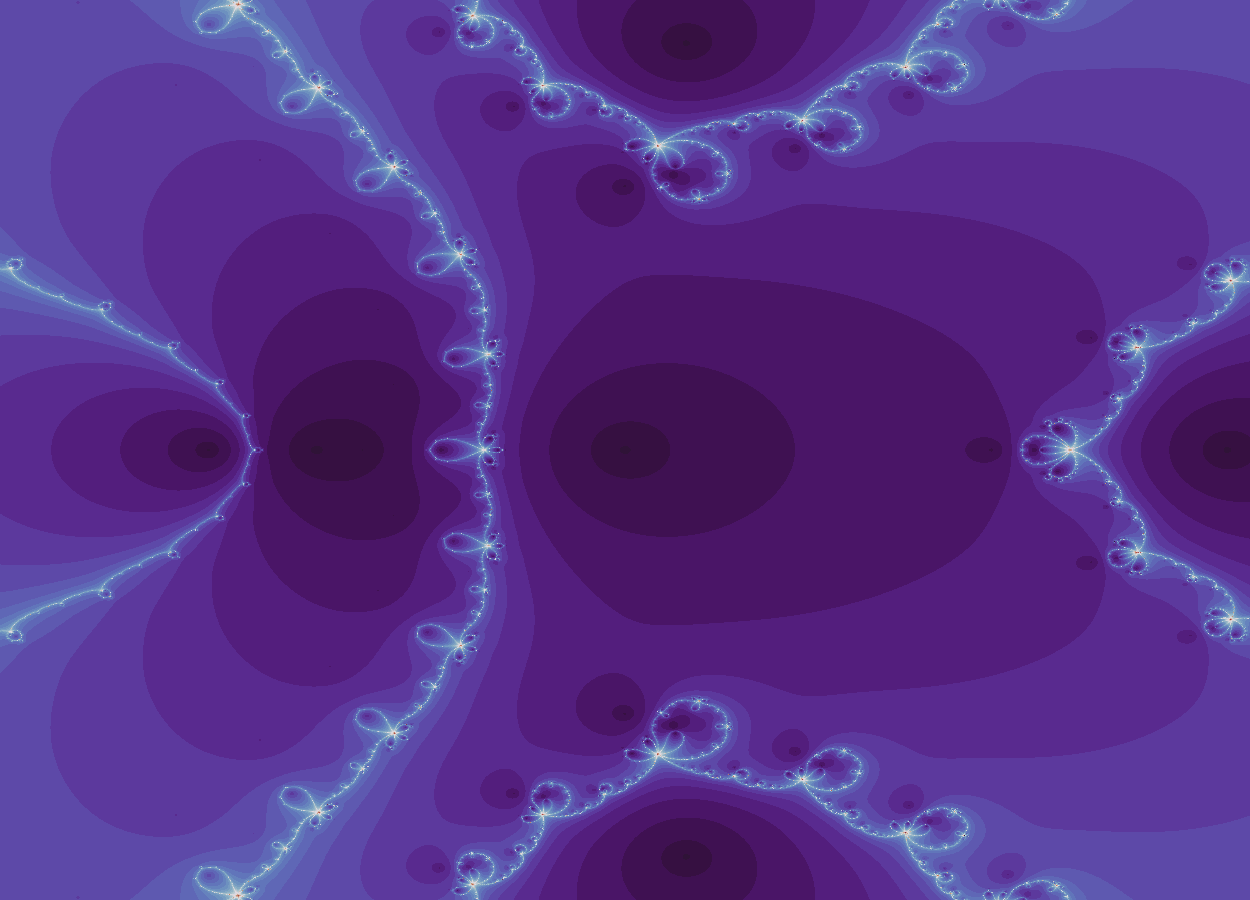
\includegraphics[scale=0.26]{images/ej4.png}
    \caption{Fractal generado por $x^6-3x^2-2x$}
    \label{fig:ej_4}
\end{figure}

\textbf{Función:}$x^7-x^2+1$

\textbf{Raíces:}

\begin{center}
\begin{tabular}{ c c  }
 (-0.8398+0i) & (-0.7555-0.7411i) \\ 
 (-0.7555+0.7411i) & (0.2945-1.0774i) \\ 
 (0.2945+1.0774i) & (0.8809-0.2758i) \\
 (0.8809+0.2758i)
\end{tabular}
\end{center}

\begin{figure}[H]
    \centering
    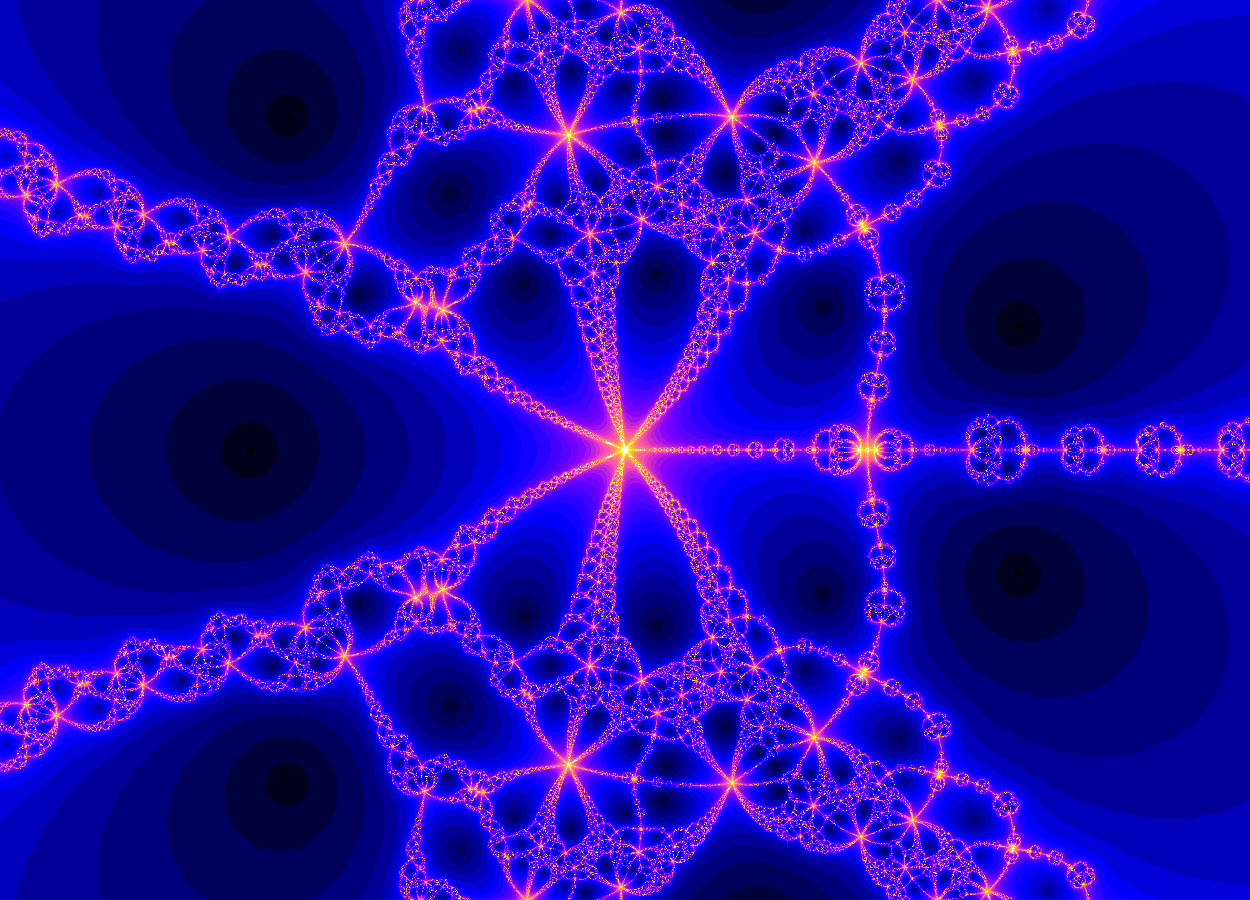
\includegraphics[scale=0.26]{images/ej5.png}
    \caption{Fractal generado por $x^7-x^2+1$}
    \label{fig:ej_5}
\end{figure}